\chapter{グラフベースSLAM}

前章まではLIOについて説明しました.
LIOを用いることで移動量を求めることができますが,移動量推定には基本的にはドリフト誤差が含まれるため,LIOで求められた移動量を基にLiDARの点群データを貼り合わせただけでは,正確な地図を構築することはできません.
正確な地図を得るためには,このドリフト誤差を補正し,点群を貼り合わせる必要があります.
本書では,これを実現するために{\bf グラフベースSLAM}(Graph-based SLAM)を用います.










\section{グラフベースSLAMの流れ}

グラフベースSLAMの実装には様々なものがありますが,本書で想定する実装の流れを最初に示します.
まず,オドメトリとマッピングの2つのプロセスを並列で起動させます.
マッピングプロセスは,オドメトリにより推定されたオドメトリ座標上のIMUの姿勢${}^{O}T_{I} \in {\rm SE}(3)$,およびこれに対応するLiDARの計測点群${}^{I}\mathcal{P}$を受け取ります.
オドメトリとしては,前章までで述べられたものが利用さることになりますので,本章ではマッピングのプロセスが行う処理の解説をします.

グラフベースSLAMにおけるマッピングプロセスでは,ノード集合$\mathcal{V}$とエッジ集合$\mathcal{E}$で構成されるグラフの作成を行います.
ここでノードとは,センサの姿勢やランドマークの位置を表すものであり,エッジはこれらのノード間の相対姿勢を表します.
ただし本書で示す実装では,ノードを用いて表すのはセンサの姿勢のみとします.
このようなグラフは{\bf ポーズグラフ}(Pose Graph)と呼ばれます.
本書で紹介するマッピングプロセスでは,このポーズグラフの構築を行い,ポーズグラフに対して定まるコスト関数の最適化を行います.

ポーズグラフ構築のために,マッピングプロセスでは,オドメトリプロセスから姿勢${}^{O}T_{I}$を受け取り,これを用いて移動量を計算していきます.
そして移動量がある一定値を超えた場合にその姿勢をキーフレーム${}^{M}T_{I}$として検出します\footnote{ キーフレームの検出にも様々な工夫をすることができますが,本書ではシンプルに移動量に対して閾値を設け,一定量移動する毎にキーフレームとして検出していきます. }.
${}^{M}T_{I, i}$が最新のキーフレームとして検出されると,キーフレームとそれに対応するLiDARの計測点群${}^{I}\mathcal{P}_{i}$を保存します.
また,オドメトリにより計算された姿勢に基づいて,2つのキーフレーム間のエッジ(オドメトリエッジ)を以下のように定めます.
%
\begin{align}
  E_{i-1, i} = {}^{O}T_{I, i-1}^{-1} {}^{O}T_{I, i}
  \label{eq:odometry_edge}
\end{align}
%

オドメトリエッジを計算した後に,{\bf ループ検知}(Loop Detection)を行います.
ループ検知とは,現在いる地点が過去に通過したことがある地点であるかどうかを識別し,過去に通過した地点であると識別されれば,今の姿勢と過去に通過した際の姿勢の間相対姿勢を認識することです.
ループ検知も様々な方法を用いて実行することが可能ですが,本書で用いる方法ではまず,新たにキーフレームとして検知された姿勢から最も近い$N$個のキーフレームを選択します.
キーフレーム間の近さを測る際には,並進ベクトルのみを用います.
そして,新しく追加されたキーフレーム,および過去に検出されたキーフレームに対応するそれぞれのLiDARの計測点群を用いて,スキャンマッチングを行います.
ループ検知におけるスキャンマッチングでは,速度より精度が重視されるため,少し計算コストが大きくなりますが,Generalized ICP(GICP)\cite{SegalRSS2009GICP}を用います.
GICPの詳細は\ref{subsec:gicp}節で述べます.
GICPによるスキャンマッチングが成功したと判定された場合に,ループ検知が行われたとしてループエッジの追加を行います.

今,最新のキーフレーム${}^{M}T_{I, i}^{'}$に対して,$j$番目のキーフレームとのGICPの結果が以下のようになったとします.
%
\begin{align}
  {}^{M}T_{I, i} = \argmin_{ {}^{M}T_{I, i}^{'} } E_{\rm GICP}({}^{M}T_{I, i}^{'}; {}^{M}T_{I, j}, {}^{I}\mathcal{P}_{i}, {}^{I}\mathcal{P}_{j})
  \label{eq:loop_detection_gicp}
\end{align}
%
ここで$E_{\rm GICP}(\cdot)$はGICPのコスト関数であり,${}^{M}T_{I, j}$,${}^{I}\mathcal{P}_{i}$,${}^{I}\mathcal{P}_{j}$は不変であるとしています.
式(\ref{eq:loop_detection_gicp})により得られた姿勢${}^{M}T_{I, i}$を用いて,ループエッジを以下のように定めます.
%
\begin{align}
  E_{i, j} = {}^{M}T_{I, i}^{-1} {}^{M}T_{I, j}
  \label{eq:loop_edge}
\end{align}
%
ループ検知を行いループエッジがエッジ集合に新たに追加されると,ポーズフラフの最適化を行います.
ポーズグラフの最適化に関しては次節で述べます.
なお,オドメトリエッジとループエッジの簡単な概略を図\ref{fig:graph_slam_residuals}に図示しています.

\begin{figure}[!t]
  \centering
  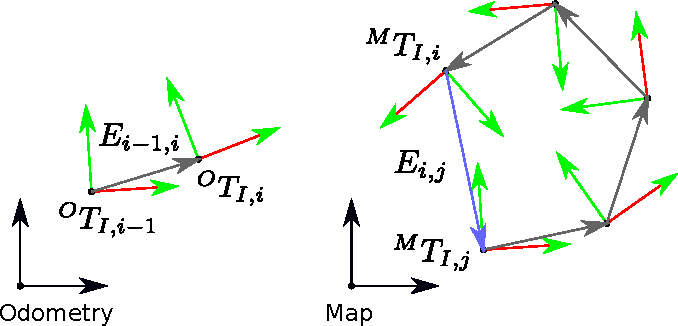
\includegraphics[width=0.5\textwidth]{../figs/graph_slam_residuals.pdf}
  \caption{Residuals used in pose graph optimization.}
  \label{fig:graph_slam_residuals}
\end{figure}
















\section{ポーズグラフの最適化}

\subsection{コスト関数}

ポーズグラフの最適化を考えるために,ポーズグラフ内で定義される残差ベクトルについて考えます.
式(\ref{eq:odometry_edge}),(\ref{eq:loop_edge})に示すように,ポーズグラフにおけるエッジは2つの姿勢間の相対姿勢として定義されます.
このエッジが観測,すなわち固定値であると仮定し,以下の残差ベクトルを定義します.
%
\begin{align}
  {\bf r}_{i, j}({}^{M}T_{I, i}, {}^{M}T_{I, j}) = \left( \log \left( E_{i, j}^{-1} {}^{M}T_{I, i}^{-1} {}^{M}T_{I, j} \right) \right)^{\vee}
  \label{eq:pose_graph_residual}
\end{align}
%
式(\ref{eq:pose_graph_residual})が$i$番目と$j$番目のエッジに対して定まる残差ベクトルとなるため,この総和を最小化する姿勢の集合を求めることでポーズグラフの最適化を行います.
%
\begin{align}
 E \left( \mathcal{T} \right) = \sum_{ i, j \in \mathcal{E} } \rho \left( \left\| {\bf r}_{i, j} \right\|_{ \Omega_{i, j} }^{2} \right)
  \label{eq:pose_graph_cost_function}
\end{align}
%
なお$\left\| {\bf r}_{i, j} \right\|_{ \Omega_{i, j} }^{2} = {\bf r}_{i, j}^{\top} \Omega_{i, j} {\bf r}_{i, j}$は情報行列$\Omega_{i, j}$を用いたマハラノビス距離の2乗を表します.





\subsection{ヤコビアンの計算}

式(\ref{eq:pose_graph_cost_function})のコスト関数を最小化するにあたり,式(\ref{eq:pose_graph_residual})に示す残差ベクトルの${}^{M}T_{I, i}$と${}^{M}T_{I, j}$に関するヤコビアンを求めます.
ヤコビアンの計算のために,$\Delta_{i, j} = E_{i, j}^{-1} {}^{M}T_{I, i}^{-1} {}^{M}T_{I, j}$を導入します.
$\Delta_{i, j}$を用いると,ヤコビアンはそれぞれ連鎖則を用いて以下のように計算できます.
%
\begin{align}
  \begin{split}
    & \frac{ \partial {\bf r}_{i, j} }{ \partial {}^{M}T_{I, i} }
    = \frac{ \partial {\bf r}_{i, j} }{ \partial \Delta_{i, j} }
      \frac{ \partial \Delta_{i, j} }{ \partial {}^{M}T_{I, i} } \\
%
    & \frac{ \partial {\bf r}_{i, j} }{ \partial {}^{M}T_{I, j} }
    = \frac{ \partial {\bf r}_{i, j} }{ \partial \Delta_{i, j} }
      \frac{ \partial \Delta_{i, j} }{ \partial {}^{M}T_{I, j} }
  \end{split}
\end{align}
%
以下,それぞれの微分について考えます.

まず$\partial {\bf r}_{i, j} / \partial \Delta_{i, j}$を考えます.
式(\ref{eq:pose_graph_residual})より,以下の等式が成り立つ$J$を求めれば良いことになります.
%
\begin{align}
  \left( \log \left( \exp \left( \delta \boldsymbol \xi^{\wedge} \right) \Delta_{i, j} \right) \right)^{\vee} - \left( \log \left( \Delta_{i, j} \right) \right)^{\vee} = J \delta \boldsymbol \xi
  \label{eq:deij_dDeltaij_J_deltaxi}
\end{align}
%
ここで$\log \left( \exp \left( \delta \boldsymbol \xi^{\wedge} \right) \Delta_{i, j} \right)$は,BCH展開を用いて以下のように1次近似することができます.
%
\begin{align}
  \left( \log \left( \exp \left( \delta \boldsymbol \xi^{\wedge} \right) \Delta_{i, j} \right) \right)^{\vee}
  \simeq {\bf r}_{i, j} + J_{l}^{-1} \left( {\bf r}_{i, j} \right) \delta \boldsymbol \xi
  \label{eq:bch_1_order_approx}
\end{align}
%
なお,${\bf r}_{i, j} = \left( \log \left( \Delta_{i, j} \right) \right)^{\vee}$であり,$J_{l}( \cdot )$は${\rm SE}(3)$に関する左ヤコビアンと呼ばれ,以下のように定義されます.
%
\begin{align}
  \begin{gathered}
    J_{l}( \boldsymbol \xi )
    = \left( \begin{matrix}
        J_{l}( \boldsymbol \phi ) & 0_{3 \times 3} \\
        Q( \boldsymbol \xi )      & J_{l}( \boldsymbol \phi ) \\
      \end{matrix} \right) \\
%
    J_{l}( \boldsymbol \phi ) = I_{3}
                              + \frac{ 1 - \cos \theta }{ \| \theta \|^{2} } \boldsymbol \phi^{\wedge}
                              + \frac{ \theta - \sin \theta }{ \| \theta \|^{3} } \left( \boldsymbol \phi^{\wedge} \right)^{2} \\
%
    Q( \boldsymbol \xi ) = \frac{1}{2} {\bf v}^{\wedge}
                         + \frac{1 - \alpha}{ \|\boldsymbol \phi \|^{2} } \left( \boldsymbol \phi^{\wedge} {\bf v}^{\wedge} + {\bf v}^{\wedge} \boldsymbol \phi^{\wedge} \right)
                         + \frac{\beta - 1}{ \|\boldsymbol \phi \|^{4} } \boldsymbol \phi^{\wedge} {\bf v}^{\wedge} \boldsymbol \phi^{\wedge} \\
%
    \alpha = \frac{ \sin \theta }{ \theta } \cdot \frac{ \theta + \sin \theta }{ 2 \left( 1 - \cos \theta \right) } \\
%
    \beta = \frac{1}{ \theta^{2} } \left( 1 - \frac{ \sin \theta }{ \theta } \right)
  \end{gathered}
  \label{eq:left_jacobian_se3}
\end{align}
%
ただし,$\boldsymbol \xi^{\wedge} = \left( \left( {\bf v}^{\top} ~ \boldsymbol \phi^{\top} \right)^{\top} \right)^{\wedge} \in \mathfrak{se}(3) $,$\boldsymbol \phi^{\wedge} \in \mathfrak{so}(3)$,$\theta = \| \boldsymbol \phi \|$です\footnote{式(\ref{eq:left_jacobian_se3})には${\rm SE}(3)$と${\rm SO(3)}$の左ヤコビアンがどちらも記載されていますが,引数が$\mathfrak{se}(3)$か$\mathfrak{so}(3)$でそれぞれを区別します.}.
式(\ref{eq:deij_dDeltaij_J_deltaxi}),(\ref{eq:bch_1_order_approx})から,$\partial {\bf r}_{i, j} / \partial \Delta_{i, j}$は以下になります.
%
\begin{align}
  \frac{ \partial {\bf r}_{i, j} }{ \partial \Delta_{i, j} } = J_{l}^{-1}( {\bf r}_{i, j} )
  \label{eq:deij_dDeltaij}
\end{align}
%

次に$\partial \Delta_{i, j} / \partial {}^{M}T_{I, i}$の微分を考えるために,まず$\Delta_{i, j} \left( \delta \boldsymbol \xi \right) = E_{i, j}^{-1} \left( \exp \left( \delta \boldsymbol \xi^{\wedge} \right) {}^{M}T_{I, i} \right)^{-1} {}^{M}T_{I, j}$,$\delta \boldsymbol \xi^{\wedge} \in \mathfrak{se}(3)$を導入します.
この$\Delta_{i, j} \left( \delta \boldsymbol \xi \right)$に左から$\Delta_{i, j}^{-1}$を掛けることで,恒等元$I_{4}$の周辺での変化量を考えます.
%
\begin{align}
  \begin{split}
    \Delta_{i, j}^{-1} \Delta_{i, j} \left( \delta \boldsymbol \xi \right)
%
    = & {}^{M}T_{I, j}^{-1} {}^{M}T_{I, i} E_{i, j} E_{i, j}^{-1} {}^{M}T_{I, i}^{-1} \exp \left( -\delta \boldsymbol \xi^{\wedge} \right) {}^{M}T_{I, j} \\
%
    = & {}^{M}T_{I, j}^{-1} \exp \left( -\delta \boldsymbol \xi \right) {}^{M}T_{I, j} \\
%
    = & \exp \left( \left( -\operatorname{Ad}_{ {}^{M}T_{I, j}^{-1} } \delta \boldsymbol \xi \right)^{\wedge} \right) \\
    \simeq & I_{4} + \left( -\operatorname{Ad}_{ {}^{M}T_{I, j}^{-1} } \delta \boldsymbol \xi \right)^{\wedge}
%
  \end{split}
\end{align}
%
式(\ref{eq:dT_dT})と比較すると,$\partial \Delta_{ij} / \partial {}^{M}T_{I, i}$は以下になることがわかります.
%
\begin{align}
  \frac{ \partial \Delta_{i, j} }{ \partial {}^{M}T_{I, i} } = - \operatorname{Ad}_{ {}^{M}T_{I, j}^{-1} }
  \label{eq:dDeltaij_dTi}
\end{align}
%

以上から,式(\ref{eq:deij_dDeltaij}),(\ref{eq:dDeltaij_dTi})より,$\partial {\bf r}_{i, j} / \partial {}^{M}T_{I, i}$は以下となります.
%
\begin{align}
  \frac{ \partial {\bf r}_{i, j} }{ \partial {}^{M}T_{I, i} } = -J_{l}^{-1}( {\bf r}_{i, j} ) \operatorname{Ad}_{ {}^{M}T_{I, j}^{-1} }
  \label{eq:deij_dTi}
\end{align}
%
なお同様の計算を行うと,$\partial {\bf r}_{i, j} / \partial {}^{M}T_{I, j}$を以下のように導くことができます.
%
\begin{align}
  \frac{ \partial {\bf r}_{i, j} }{ \partial {}^{M}T_{I, j} } = J_{l}^{-1}( {\bf r}_{i, j} ) \operatorname{Ad}_{ {}^{M}T_{I, i} }
  \label{eq:deij_dTj}
\end{align}



\subsection{ガウス・ニュートン法による最適化}

式(\ref{eq:pose_graph_cost_function})に示すコスト関数を最小化するためにも,ガウス・ニュートン法を用います.
まず式(\ref{eq:pose_graph_residual})に示す残差ベクトル${\bf r}_{i, j}$に対する${}^{M}T_{I, i}$,および${}^{M}T_{I, j}$に関するヤコビアンは,それぞれ式(\ref{eq:deij_dTi}),(\ref{eq:deij_dTj})のように定まります.
以下,それぞれのヤコビアンを$J_{i}$,$J_{j}$とします.
今,$i, j$番目のエッジに対して定まる残差ベクトル${\bf r}_{i, j}$に対するヤコビアンを$J_{i, j} = \left( 0 ~ \cdots ~ 0 ~ J_{i} ~ 0 ~ \cdots 0 ~ J_{j} ~ 0 ~ \cdots ~ 0 \right) \in \mathbb{R}^{6 \times 6N}$とします($i, j$番目の残差に影響を与えるのは$i$,$j$番目の姿勢のみのため,それ以外の要素はすべて0になります.).
これを用いて,ヘッセ行列$H \in \mathbb{R}^{6N \times 6N}$,と勾配ベクトル${\bf b} \in \mathbb{R}^{6N}$を求めます.
%
\begin{align}
  \begin{gathered}
    H = \sum_{ ij \in \mathcal{E} } w_{i, j} J_{i, j}^{\top} J_{i, j} \\
    {\bf b} = \sum_{ ij \in \mathcal{E} } w_{i, j} J_{i, j}^{\top} {\bf r}_{i, j} \\
  \end{gathered}
  \label{eq:graph_slam_hessian_gradient}
\end{align}
%
なお,$w_{i, j} = \rho^{\prime} \left( \| {\bf r}_{i, j} \|_{ \Omega_{i, j}^{2} } \right)$です.
このヘッセ行列と勾配を用いて,$H \delta \boldsymbol \xi = -{\bf b}$を満たす$\delta \boldsymbol \xi$を求めます.
$\delta \boldsymbol \xi \in \mathbb{R}^{6N}$は$N$個のブロックで構成されるベクトルとなっており,各ブロックはそれぞれの姿勢に対応する更新量となっています.
つまり$i$番目のブロックのベクトルを$\delta \boldsymbol \xi_{i} \in \mathbb{R}^{6}$とすると,対応する$i$番目の姿勢${}^{M}T_{I, i}$は以下のように更新されます.
%
\begin{align}
  {}^{M}T_{I, i} \leftarrow \exp \left( \delta \boldsymbol \xi_{i}^{\wedge} \right) {}^{M}T_{I, i}
\end{align}
%

グラフベースSLAMを実装するにあたり,ヘッセ行列のサイズは$6N \times 6N$となり,単純に逆行列を求めると計算コストが非常に大きくなってしまいます.
しかし多くの場合,一般的なグラフベースSLAMでは,$H$の対角成分以外のほとんどの成分が0となります.
このような行列は{\bf 疎行列}(Sparse Matrix)と呼ばれ,専用のソルバーを用いると高速に$H \delta \boldsymbol \xi = -{\bf b}$を満たす$\delta {\bf x}$を求めることができます.
そのため,実際には式(\ref{eq:graph_slam_hessian_gradient})に示すような大きなサイズのヤコビアンの計算は行わず,$J_{i}$,$J_{j}$を計算して,行列の各要素に加算していくような計算を行います.













\section{ループ検知}
\label{subsec:gicp}

\subsection{GICPの最適化}

前述の通り,ループ検知のためにはGICPを用います.
GICPはSource点群$\mathcal{P}$とTarget点群$\mathcal{Q}$の2つの点群を照合するために利用できる手法です.
GICPでは,それぞれの点群を正規分布を用いて表現しますが,そのためにまず,各点群の全ての点に対して最近某探索を行い,各点群内から周辺の点を取得します.
そしてそられの点を用いて,平均と共分散行列を計算します.
平均と分散の計算は式(\ref{eq:points_mean}),(\ref{eq:points_covariance})に基づきます.
すなわち,$\mathcal{P}$の$i$番目の点は$\bar{ {\bf p} }_{i}$と$C_{i}^{p}$,$\mathcal{Q}$の$i$番目の点は$\bar{ {\bf q} }_{i}$と$C_{i}^{q}$によりそれぞれ表されます.
GICPでは,これらを用いてコスト関数を以下のように定めます.
%
\begin{align}
  E \left( T \right) = \sum_{i=1}^{N} \rho \left( \left( \bar{ {\bf q} }_{i} - T \bar{ {\bf p} }_{i} \right)^{\top} \left( \hat{C}_{i}^{q} + T \hat{C}_{i}^{p} T^{-1} \right)^{-1} \left( \bar{ {\bf q} }_{i} - T \bar{ {\bf p} }_{i} \right) \right)
  \label{eq:gicp_cost_function}
\end{align}
%
ただし$\hat{C}^{p}$,$\hat{C}^{q}$は以下となります.
%
\begin{align}
  \begin{gathered}
    \hat{C}^{p} = \left( \begin{matrix}
      C^{p}          & {\bf 0} \\
      {\bf 0}^{\top} & 0
    \end{matrix} \right) \in \mathbb{R}^{4 \times 4} \\
%
    \hat{C}^{q} = \left( \begin{matrix}
      C^{q}          & {\bf 0} \\
      {\bf 0}^{\top} & 0
    \end{matrix} \right) \in \mathbb{R}^{4 \times 4}
  \end{gathered}
\end{align}
%

\begin{figure}[!t]
  \centering
  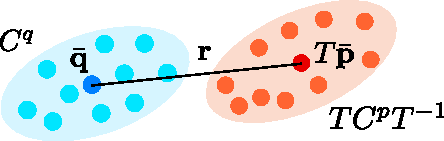
\includegraphics[width=0.3\textwidth]{../figs/gicp_residual.pdf}
  \caption{Residual error used in GICP.}
  \label{fig:gicp_residual}
\end{figure}


本書では,GICPもガウス・ニュートン法を用いて解きますが,表記の簡略化のために,${\bf r}_{i} = \bar{ {\bf q} }_{i} - T \bar{ {\bf p} }_{i}$,$\Omega_{i} = \left( \hat{C}_{i}^{q} + T \hat{C}_{i}^{p} T^{\top} \right)^{-1}$とおきます.
まず${\bf r}_{i}$の$T$に対するヤコビアンを求めるために,以下を満たす$J_{i}$を求めます.
%
\begin{align}
  \bar{ {\bf q} }_{i} - \exp \left( \delta \boldsymbol \xi^{\wedge} \right) T \bar{ {\bf p} }_{i} - \left( \bar{ {\bf q} }_{i} - T \bar{ {\bf p} }_{i} \right) = J_{i} \delta \boldsymbol \xi
  \label{eq:gicp_jacobi_approx}
\end{align}
%
式(\ref{eq:gicp_jacobi_approx})の左辺を展開すると,以下が得られます.
%
\begin{align}
  \begin{split}
    -\exp \left( \delta \boldsymbol \xi^{\wedge} \right) T \bar{ {\bf p} }_{i} + T \bar{ {\bf p} }_{i}
%
    = & - \left( \exp \left( \delta \boldsymbol \xi^{\wedge} \right) - I_{4} \right) T \bar{ {\bf p} }_{i} \\
%
    = & - \left( \begin{matrix}
            \delta \boldsymbol \phi^{\wedge} & \delta {\bf v} \\
            {\bf 0}^{\top}                   & 0
          \end{matrix} \right)
          \left( \begin{matrix}
            \bar{ {\bf p} }_{i}^{'} \\
            1
          \end{matrix} \right) \\
%
    = & - \left( \begin{matrix}
            - \left( \bar{ {\bf p} }_{i}^{'} \right)^{\wedge} \delta \boldsymbol \phi + \delta {\bf v} \\
            0
          \end{matrix} \right) \\
%
    = & \left( \begin{matrix}
          -I_{3}         & \left( \bar{ {\bf p} }_{i}^{'} \right)^{\wedge} \\
          {\bf 0}^{\top} & {\bf 0}^{\top}
        \end{matrix} \right) \delta \boldsymbol \xi \\
  \end{split}
\end{align}
%
ただし,$\bar{ {\bf p} }_{i}^{'} = R \bar{ {\bf p} }_{i} + {\bf t}$としています.
よって,式(\ref{eq:gicp_jacobi_approx})を満たす$J_{i}$は以下になります.
%
\begin{align}
  J_{i} = \left( \begin{matrix}
            -I_{3}         & \left( \bar{ {\bf p} }_{i}^{'} \right)^{\wedge} \\
            {\bf 0}^{\top} & {\bf 0}^{\top}
          \end{matrix} \right)
  \label{eq:gicp_jacobian}
\end{align}
%
このヤコビアンを用いて,ヘッセ行列と勾配を以下のように求めます.
%
\begin{align}
  \begin{gathered}
    H = \sum_{i=1} w_{i} J_{i}^{\top} \Omega_{i} J_{i} \\
    {\bf b} = \sum_{i=1} w_{i} J_{i}^{\top} \Omega_{i} {\bf r}_{i} \\
  \end{gathered}
  \label{eq:gicp_hessian_and_gradient}
\end{align}
%
なお$w_{i} = \rho^{\prime} \left( {\bf r}_{i} \Omega_{i} {\bf r}_{i} \right)$です.
この$H$と${\bf b}$を用いて,$H \delta \boldsymbol \xi = -{\bf b}$を満たす$\delta \boldsymbol \xi$を求め,$T \leftarrow \exp \left( \delta \boldsymbol \xi^{\wedge} \right) T$で姿勢を更新します.

式(\ref{eq:gicp_hessian_and_gradient})の導出について簡単に述べますが,これは\ref{subsec:gauss-newton_method}節でも述べたように,状態が微小変化した際の残差ベクトルの線形近似を用いたコスト関数について考えることで導出できます.
%
\begin{align}
  \sum_{i=1}^{N} \left( {\bf r}_{i} + J_{i} \delta \boldsymbol \xi \right)^{\top} \Omega_{i} \left( {\bf r}_{i} + J_{i} \delta \boldsymbol \xi \right)
  =
  \sum_{i=1}^{N} {\bf r}_{i}^{\top} \Omega_{i} {\bf r}_{i} + 2 \delta \boldsymbol \xi^{\top} \Omega_{i} J_{i} {\bf r}_{i} + \delta \boldsymbol \xi^{\top} J_{i}^{\top} \Omega_{i} J_{i} \delta \boldsymbol \xi
\end{align}
%
この右辺を$\delta \boldsymbol \xi$で微分して{\bf 0}とすると以下が得られます(ただし式(\ref{eq:gicp_hessian_and_gradient})と比較して,下の式では$w_{i}$が抜けていることに注意してください).
%
\begin{align}
  \sum_{i=1}^{N} J_{i}^{\top} \Omega_{i} J_{i} \delta \boldsymbol \xi = -\sum_{i=1}^{N}  J_{i}^{\top} \Omega_{i} {\bf r}_{i}
\end{align}
%



\subsection{ループ検知の成功判定}

ループ検知のためにGICPを用いて,式(\ref{eq:gicp_cost_function})に示すコスト関数の最小化を行い,点群の照合を行います.
この照合結果を基にループ検知の成功・失敗を判断する必要があるのですが,点群の照合の是非を明示的に示す指標を作成することは困難です.
例えば,最終的なコスト関数の値,もしくは残差の平均値が一定以下になっているというような閾値は,ある程度の精度で照合の是非を判定できますが,必ずしも判断の正しい指標になるとはいえません.
しかし実装においては,これらの指標を用いるのが有用な場合が多くあります.
本書で紹介している実装では,残差の平均値や,照合率(最近傍点との距離が閾値以下の点の割合)などに閾値を定め,これらに基づきループ検知が成功したかどうかの判定を行っています.

ただしこのような方法では,照合に失敗した場合でも成功したと判定してしまう場合があります.
このような誤った情報がグラフに組み込まれると,グラフの最適化が破綻してしまうこともあります.
そのため式(\ref{eq:graph_slam_hessian_gradient})に示すように,グラフの最適化においてもフーバー損失等のロバストカーネルを利用することが有効になります.











\section{座標変換の計算と地図構築}

\subsection{座標変換}

LIOを用いると,オドメトリ座標上でのIMUの姿勢${}^{O}T_{I}$が得られます.
またポーズグラフの最適化を実行すると,新しく検出されたキーフレームの位置が修正され,それが地図座標上でのIMUの姿勢${}^{M}T_{I}$となります.
この2つの姿勢を用いて,図\ref{fig:frames}に示す地図とオドメトリ座標間の変換${}^{M}T_{O}$を求めるにあたり,図\ref{fig:map_odom_transformation}ように,地図座標上のIMUの姿勢,およびオドメトリ座標上でのIMUの姿勢が一致するとします.
するとこの関係から,${}^{M}T_{O}$を以下のように求められます.
%
\begin{align}
  \begin{split}
    {}^{M}T_{O} = & {}^{M}T_{I} {}^{O}T_{I}^{-1} \\
                = & {}^{M}T_{I} {}^{I}T_{O}
  \end{split}
\end{align}
%
なお本書で詳細は述べませんが,自己位置推定をする場合でも同じように${}^{M}T_{O}$を求めます.

\begin{figure}[!t]
  \centering
  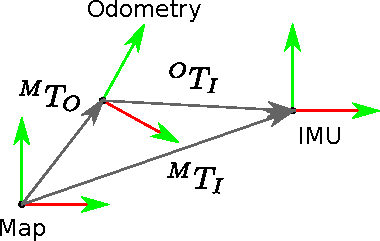
\includegraphics[width=0.3\textwidth]{../figs/map_odom_transformation.pdf}
  \caption{Residuals used in pose graph optimization.}
  \label{fig:map_odom_transformation}
\end{figure}



\subsection{地図構築}

ポーズグラフの最適化が終わると,地図座標上での各キーフレームが${}^{M}T_{I, i}$修正されます.
これらの姿勢,および各キーフレームに対応する点群${}^{I}\mathcal{P}_{i}$を用いて,以下のように点群地図を構築します.
%
\begin{align}
  {}^{M}\mathcal{M} = \bigcup_{i=1}^{K} \bigcup_{{}^{I}{\bf p} \in {}^{I}\mathcal{P}_{i}} {}^{M}T_{I, i} {}^{I}{\bf p}
\end{align}
%
ここで$K$はキーフレームの数です.
ただし本書で紹介しているグラフベースSLAMでは,この地図点群が処理に利用されることはありません.
そのため,SLAMプロセス終了時に一度実行するだけでも問題はありません.
ポーズグラフの最適化後に都度実行すると,地図が正しく構築できているかをオンラインで確認することができるため,本書で紹介する実装では最適化後に毎回実行しています.





\section{実用にあたって}

本章で紹介した方法では,移動量に対して閾値を設けてキーフレームを検出し,そのキーフレームに対応するLiDARの観測点群を保存しておき,この点群をキーフレームに合わせて座標変換することで地図の作成を行いました.
この方法を採用すると,LiDARが計測した全ての点群を用いて地図の作成を行わくなるため,地図点群の密度が低下するという問題が発生してしまいます.
点群の密度を上げるために,例えば一定時間LiDARの計測点群を蓄積したらキーフレームとして検出するという方法も考えられますが,この方法を用いると時間経過とともに使用するメモリ容量が増大してしまいます.
一方で移動量に対して閾値を設けてキーフレームを検出する方法であれば,移動量に対してメモリ容量が増大するため,メモリ効率は優れるというトレードオフがあります.


もし単に点群密度の高い地図を作りたというだけであれば,SLAMを用いて地図を作成した際に使用した同じデータを用いて,その地図上で再度位置推定を実行し,その位置推定結果を基に点群をマッピングするという方法もあります.
少し面倒にはなりますが,この方法であればメモリコストを気にせずに高密度の点群地図が作成することができます.
ただし点群データの全体的な整合性を考えてマッピングされた結果とはならないため,確実に正確な地図が得られる保証がないことには留意しなければなりません.

本章で紹介した方法は,ポーズグラフを用いたグラフベースSLAMになります.
ポーズグラフを用いる場合,LiDARの点群データは最適化対象にならなくなるため,マッピングの精度は通常のグラフベースSLAMと比較すると低下してしまいます.
ただし,通常グラフベースSLAMでは,メモリコストの問題があるため,LiDARが計測した点群すべてを最適化対象にはせず,特徴点やランドマークをLiDARの点群から検出し,これらの位置を最適化対象に加えます.
そのため,特徴点やランドマークの検出性能,またそれらの対応付けの性能がマッピングの精度にも影響することになります.
近年の3D LiDARは観測距離も長く,点群の密度も高いため,単純に2つの計測データを照合するだけでも,高い精度で相対位置を知ることができます.
そのため,このような前提であれば,ポーズグラフの最適化だけでも十分な精度の地図を得られることが多いです.
ただし,文献\cite{}に見られるように,地図全体を最適化するというプロセスを踏むと,より地図の精度を向上させることもできるため,ポーズグラフの最適化だけで十分な精度が得られるかどうかはケースバイケースであるといえます.

本章で述べた方法では,ループ検知を行うために,単純に近隣のキーフレーム間でスキャンマッチングを行うという方法を用いています.
\ref{sec:scan_matching_実用にあたって}でも述べましたが,スキャンマッチングが正しく機能する前提の1つに初期姿勢がある程度正確に取得できてることが挙げられます.
ただしオドメトリでは,移動に対する累積(ドリフト)誤差が無視できないため,SLAM実行中の移動量が長くなるにつれ,ループ検知を行うためのスキャンマッチングの初期姿勢の精度が低下してしまいます.
そのため,単純にスキャンマッチングを用いてループ検知を行うだけでは,大きなループを閉じることができない場合もあります.
そのような場合には,例えばLiDARの計測点群から特徴点や特徴量を抽出し,複数の点群から類似性の高い点群を検出するという方法を用いなければなりません.
ただしこのような方法は,スキャンマッチングでループを検出するより,一般的に精度が低下してしまうことが多いです.
そのため,ポーズグラフの最適化時におけるアウトライアの検出なども考慮する必要が発生することもあります.

なおスキャンマッチングを用いてループ検出を行う場合だけでも,正しくループが閉じることができてれば,オドメトリによる累積誤差が補正できていることを意味します.
そのため,ループが閉じやすいような経路を考えてデータを取得することで,地図作成を成功させるということも実用的にはあります.
ただしループが大きすぎる場合は性能の限界があるため,違う方法の導入を検討しなければなりません.





